\graphicspath{{content/chapters/3_literature/figures/}}
\chapter{Literature Review}
\label{sec:literature_review}

This chapter reviews the key literature that directly informed the design and implementation of the project. While many aspects of the system drew on established methods and architectures, the following discussion focuses on the most influential and relevant papers. Three core areas are covered: handling variable-length sequences in datasets, the application of fully convolutional neural networks (FCNs) for speech enhancement, and the Conv-TasNet architecture for end-to-end speech separation.

\section{Distortion Free Variable Length Handling} 
\label{sec:distortion_free_handling}

A significant challenge addressed in Section~\ref{sec:variable_length_handling} is the handling of variable-length audio sequences within the dataset. To identify suitable strategies, a review of relevant research was conducted, with the method proposed by Yoon and Yu~\cite{yoon2020pto} emerging as particularly applicable.

Their work focuses on minimizing the information distortion introduced when sequences of varying lengths are batched for training. They explain the shortcomings of traditional padding and truncation methods, as well as more advanced implementations such as \texttt{PackedSequence} in PyTorch. While these methods enable batch processing, they inevitably introduce either loss of important information (via truncation) or addition of irrelevant information (via padding).

To address this, Yoon and Yu proposed the Padding-Truncation Output-Truncation (PTO) method, a distortion-free technique that preserves the original sequence structure. In PTO, sequences are padded within a batch to match the longest input, but after processing, outputs are truncated back to their respective original lengths.

Experimental evaluation on the RSR2015 speaker verification dataset demonstrated that the PTO method consistently outperformed conventional approaches in terms of equal error rate (EER), achieving up to a 27\% relative improvement over baseline methods, while incurring only a modest computational overhead.

Given its distortion-free nature and suitability for real-time speech enhancement, PTO was adopted in this project as one of the three primary methods for handling variable-length sequences. It is further discussed in Section~\ref{subsec:pto_dataset} and evaluated in Section~\ref{sec:dataset_performance}.

\section{Fully Convolutional Neural Network Adaptations}
\label{sec:fcns}

When considering the model architectures for the speech enhancement system, extensive research was conducted into models specifically designed for denoising tasks. Beyond standard CNN and U-Net architectures already established in the field, the focus was placed on identifying designs that innovated.

One particularly relevant work is the study by Park and Lee~\cite{park2017acoustic}, which proposed the use of fully convolutional neural networks for speech enhancement. Two architectures are displayed here, the CED and its improved variant, the R-CED, both specifically designed for the task of speech enhancement and operating directly on spectrogram data.

The CED model follows a symmetric encoder-decoder structure without an explicit bottleneck and is optimized for temporal feature extraction using frequency-preserving convolutional kernels. The real and imaginary components of the spectrogram are concatenated to form a two-channel input. The network compresses input features along the encoder and reconstructs them along the decoder, using pooling and upsampling operations to manage feature dimensions.

However, the paper notes a drawback of the CED architecture. Aggressive compression and upsampling operations can lead to information loss, particularly in the context of speech signals where temporal resolution is critical. To address this, the authors proposed the R-CED model. It removes pooling and upsampling layers entirely, instead employing redundant convolutional layers to augment feature representations. This design maintains full resolution throughout the network, enabling more effective denoising without sacrificing temporal fidelity.

\begin{figure}[H]
    \centering
    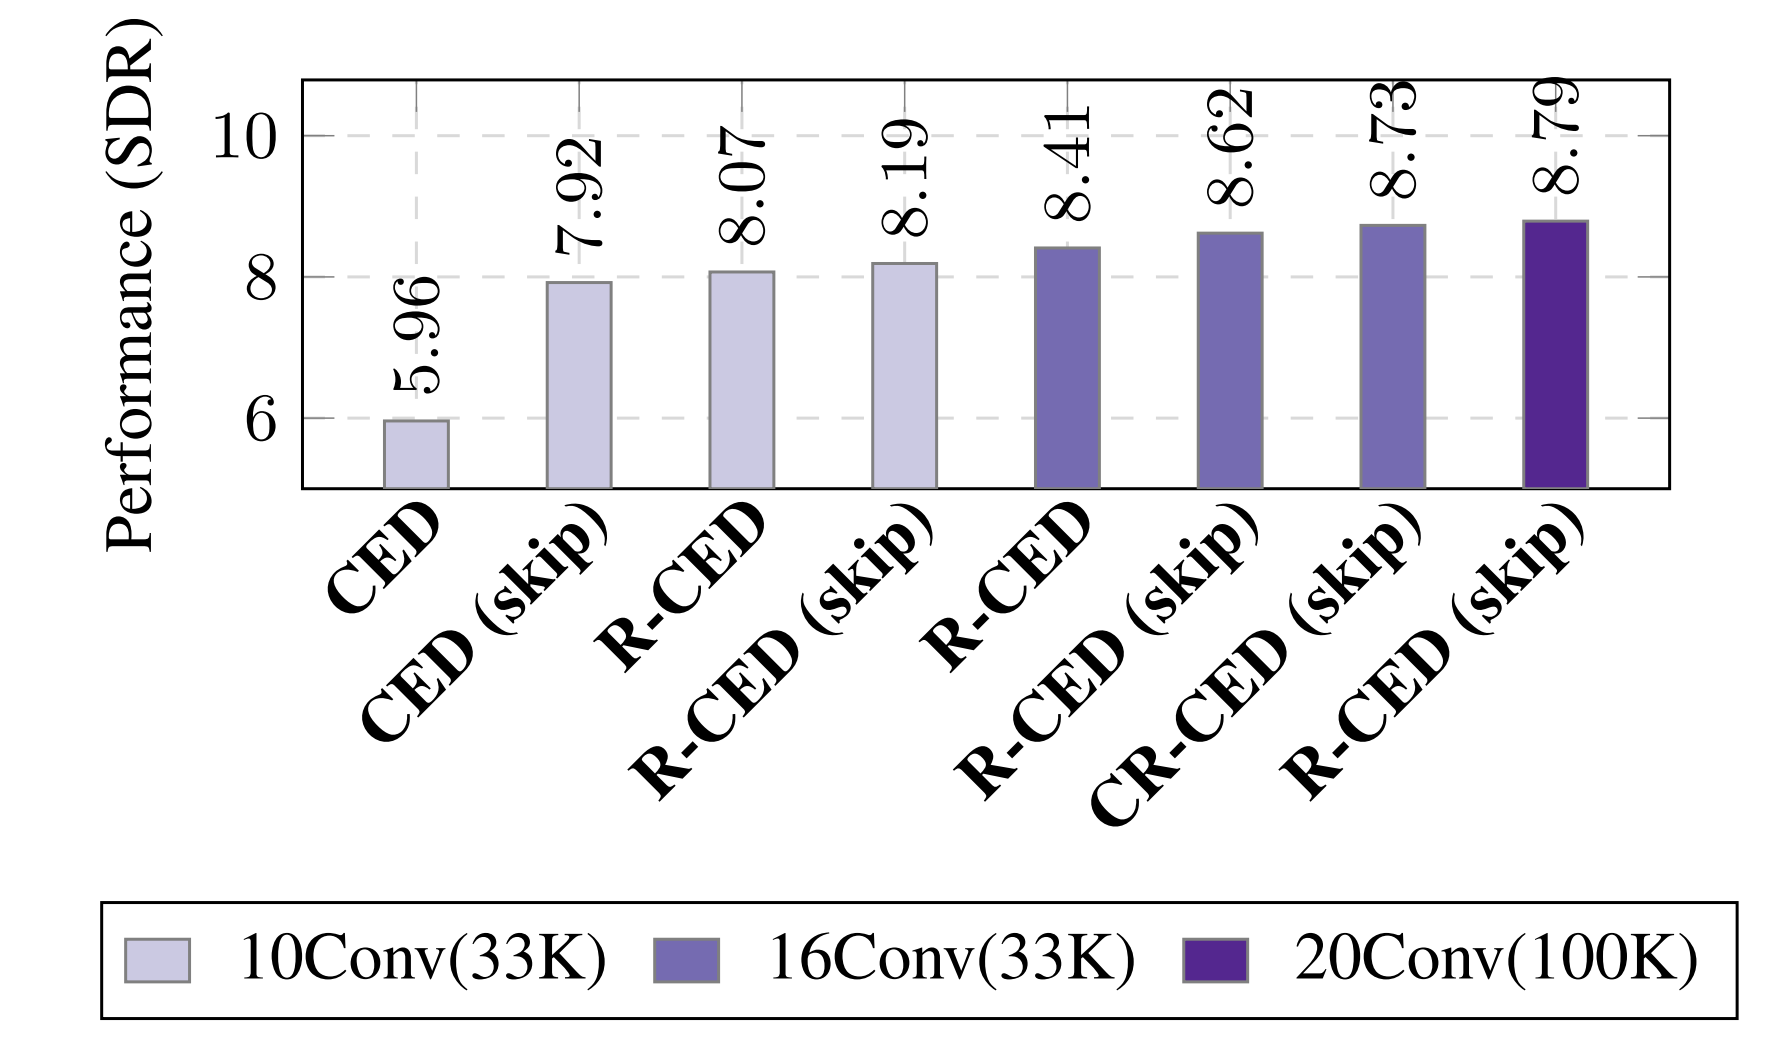
\includegraphics[width=0.8\textwidth]{CED_RCED.png}
    \caption{A Comparison of Denoising Performance and the
    Model Size for different CNN Architectures \cite{park2017acoustic}.}
    \label{fig:fcns_results}
\end{figure}

The results of the study demonstrated that R-CED consistently outperformed the conventional CED when evaluated with 10 convolutional layers and an equal parameter budget. Furthermore, performance improvements were observed by incorporating skip connections between encoder and decoder layers, which allow low-level feature information to be preserved and passed through the network. As shown in Figure~\ref{fig:fcns_results}, the addition of skip connections further enhanced the denoising capability of both the CED and R-CED architectures, with the R-CED (skip) configuration achieving the highest overall performance among the tested models.


\section{Conv-TasNet for End-to-End Speech Separation}
\label{sec:convtasnet_lit_review}

Conv-TasNet is a convolutional neural network architecture proposed by Luo and Mesgarani~\cite{luo2019conv}, representing a significant advancement in the field of speech enhancement. Unlike traditional approaches that operate in the time-frequency domain, Conv-TasNet processes raw audio waveforms directly using a Temporal Convolutional Network (TCN). The TCN replaces recurrent layers by employing stacked dilated convolutions and residual connections, enabling efficient modeling of long-range temporal dependencies with fewer layers.

Each TCN block consists of a depthwise separable convolution, non-linear activation (PReLU), normalization (group normalization), and a residual connection. Dilation factors increase exponentially across layers (e.g., 1, 2, 4, 8), allowing the model to expand its receptive field efficiently while maintaining computational stability. By stacking multiple TCN blocks, Conv-TasNet captures broad temporal contexts without the sequential limitations of recurrent models.

Conv-TasNet achieved state-of-the-art performance in speech separation tasks, surpassing conventional magnitude masking methods. The paper demonstrated the model's ability to separate multiple overlapping speakers from a single-channel recording under challenging conditions, highlighting the effectiveness of its end-to-end training approach in learning optimal source representations.

\begin{figure}[H]
    \centering
    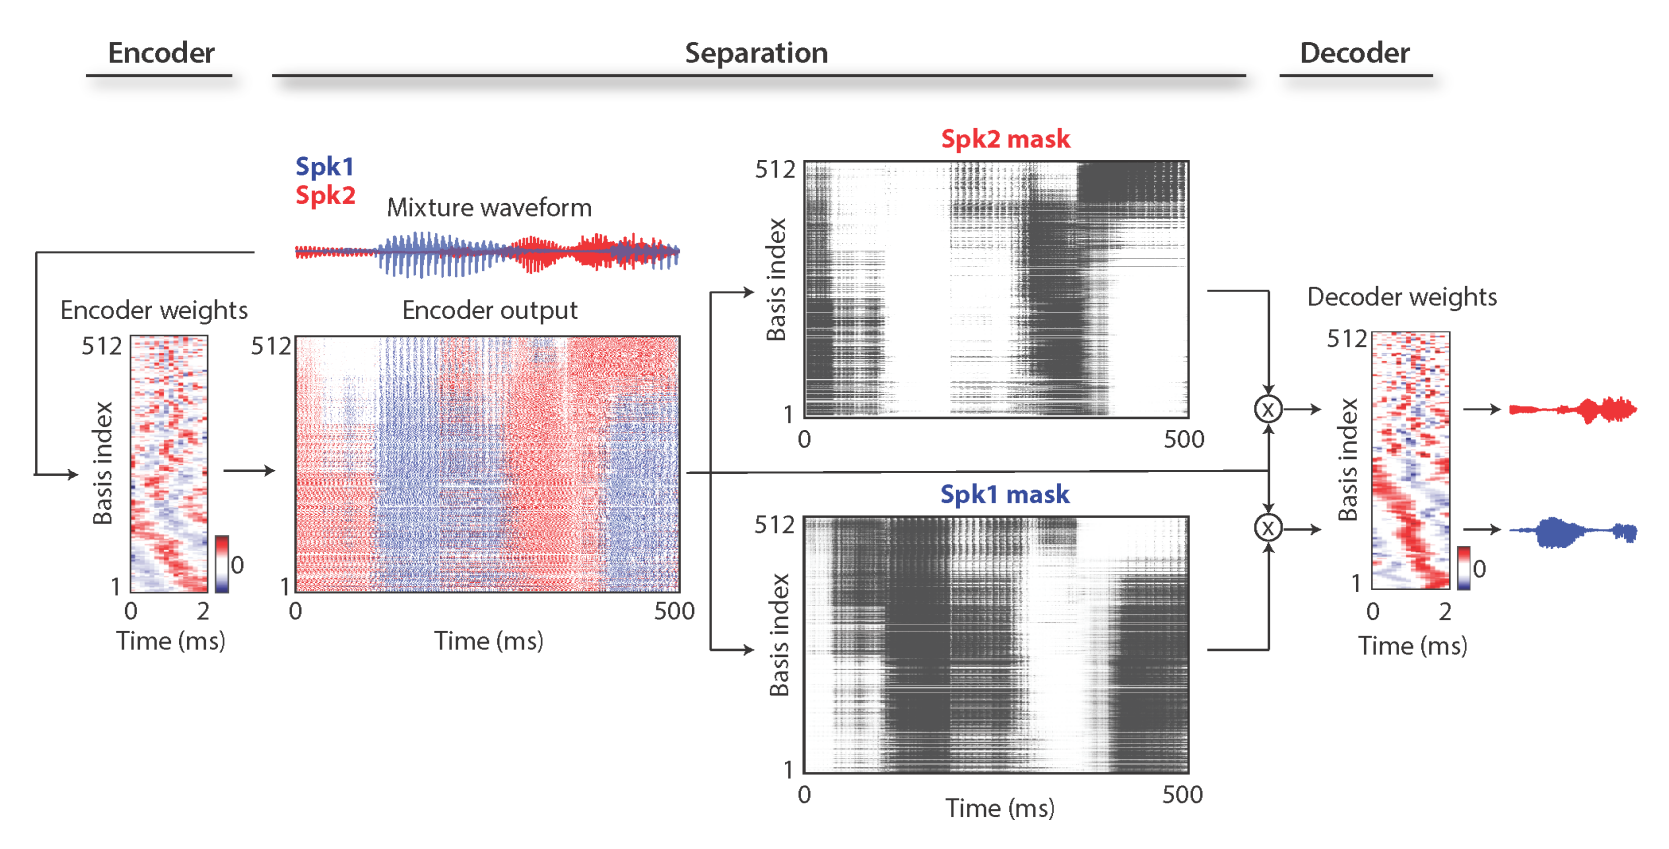
\includegraphics[width=0.8\textwidth]{TwoSpeakSeperation.png}
    \caption{Source masks for a sample two-speaker mixture \cite{luo2019conv}.}
    \label{fig:convtasnet}
\end{figure}

In this project, the Conv-TasNet framework is adapted to operate on complex-valued spectrogram inputs for the task of speech denoising, while preserving the Temporal Convolutional Network (TCN) structure for modeling long-range dependencies.
